\documentclass{article}
\usepackage{graphicx}
\usepackage{listings}
\usepackage{xcolor}
\usepackage{makeidx}
\usepackage{amsmath, amsthm, amssymb}

\lstdefinestyle{myCsharpstyle}{language=[Sharp]C,backgroundcolor=\color{gray!10}, keywordstyle=\color{blue},commentstyle=\color{green!40!black},stringstyle=\color{orange},basicstyle=\footnotesize\ttfamily, breaklines=true, tabsize=4, columns=fullflexible, showstringspaces= false, escapeinside={(*@}{@*)}, }


\makeindex
\begin{document}

\lstset{style=myCsharpstyle}
\begin{center}
\Huge\textbf{Primer Proyecto de Programación Moogle}\\
\vspace{0.5em}
\large Olivia Ortiz Arboláez \\
\tiny Julio de 2023
\end{center}

Para hacer este proyecto, requerí un proceso de investigación sobre distintas utilidades además de una planificación 
y puesta en práctica de las mismas tal que se adaptasen al objetivo de hacer un código en C\# para un buscador.

\index{Inicio}
\index{Cargar Documentos}


\section{Inicio} 

\subsection{Cargar los Documentos}
Claro, para que el buscador funcione tiene que leer los archivos que estén dentro de una carpeta. Ese sería el primer paso.
En la clase Program del proyecto se crea un objeto \textbf{DB} tipo \textcolor{purple}{Database}, que es una clase que posee varias propiedades. Dichas propiedades servirán para trabajar con los archivos
que compondrán la base de datos del buscador.

\begin{lstlisting}
    
(*@\textcolor{blue}{using }@*)System ;
(*@\textcolor{blue}{using }@*)System.IO ;

public class (*@\textcolor{purple}{Database}@*)
{
    public (*@\textcolor{green}{Document}@*)[] docs ;
}


\end{lstlisting}

Como se puede ver en este código, la clase \textcolor{purple}{Database} posee un array tipo \textcolor{green}{Document} llamado docs.\\
\setlength Todos los objetos tipo \textcolor{green}{Document} tienen la propiedad ruta en dicha clase. Por tanto el array contendrá constancia de dicha propiedad en cada elemento que posea.

Ahora bien, es momento de cargar los documentos. Para ello fue empleada la siguiente función:

\begin{lstlisting}
      private void CargarDocs(string folder)
    {
        IEnumerable <string> Verarchivos = Directory.EnumerateFiles (folder , "*.txt" , SearchOption.AllDirectories) ;
        this.docs = new Document[Verarchivos.Count()] ;
       
        Parallel.For(0 , docs.Length , i => 
        {
            this.docs[i] = new Document(Verarchivos.ElementAt(i)) ;           
        });

    }
\end{lstlisting}

Esta función no hace más que leer los archivos .txt que se encuentran en la carpeta que se le es pasada por parámetro y, por cada 
archivo que encuentra la función \textcolor{green!40!black}{EnumerateFiles} crea un nuevo objeto tipo documento que es enviado hacia el array docs mediante un bucle.

Quedando como elementos de docs[] los archivos .txt que están en la carpeta\footnote{La carpeta de ejemplo empleada tenia de nombre Content, pero para generalizar se utiliza folder.} 

\subsection{Almacenar datos}
Teniendo ya constancia de cada documento que será empleado para la futura búsqueda, estamos en disposición de guardar las palabras contenidas en cada uno de ellos. Para esto transité por un 
postergado proceso de análisis acerca de cuál sería la forma más conveniente para dicha tarea.\footnote{Varias ideas cruzaron por mi mente: la creación de un array para que fuesen almacenadas las palabras, una lista o lo empleado finalmente para este propósito,un diccionario. }
\\En este caso:\\
\begin{lstlisting}
    public Dictionary <string , Dictionary <int , int> > \textcolor{yellow}{contenido} = new Dictionary <string , Dictionary <int , int> > () ;  

\end{lstlisting}

Siendo este diccionario \textcolor{yellow!80!black}{\textcolor{yellow}{contenido}} una propiedad de \textcolor{purple}{Database} y un diccionario de diccionarios, puesto que tendría por cada palabra que se le asigne, un diccionario de enteros asociado a esta. Este diccionario de enteros subordinado busca contener como Key documentos donde se encuentra la palabra y como Value la cantidad de veces que se halla en el documento actual.\\
\textbf{Ejemplo: (Cactus, (1 , 4 ) ) }\\


Pues, para que la búsqueda sea más eficiente, es necesario estandarizar las palabras que están en estos documentos, quitando problemáticas futuras como diferencias entre letras mayúsculas, minúsculas y acentos que pueden ser a veces simples errores humanos de escritura. Para esto empleé una función llamada \textcolor{cyan}{Estandarizador} en la clase \textcolor{magenta}{Xtra}.
Esta clase \textcolor{magenta}{Xtra} posee métodos variados de utilidad que serán llamados conforme vayan siendo necesitados.

A continuación la función \textcolor{orange}{FillDict}.

\begin{lstlisting}
   private void FillDict ()
    {
        for (int i = 0; i < docs.Length; i++)
        {
            string[] text = Xtra.Estandarizador( File.ReadAllText( docs[i].ruta)).Split() ;
                
            foreach (string word in text )
            {
                if ( ! this.\textcolor{yellow}{contenido}.ContainsKey(word) )
                {
                    this.\textcolor{yellow}{contenido}.Add( word , new Dictionary <int , int> ()  ) ;
                }
                
                if (! \textcolor{yellow}{contenido}[word].ContainsKey(i) )
                {
                    \textcolor{yellow}{contenido}[word].Add(i , 0);
                }
                
                \textcolor{yellow}{contenido}[word][i]++ ;
            }
        }
    }

\end{lstlisting}


La misma lee las palabras que hay en los documentos según la ruta, separa estas palabras, las estandariza y las coloca en un array tipo string. Luego toma estas palabras y las añade al
diccionario \textcolor{yellow!80!black}{\textcolor{yellow}{contenido}} si no están y el documento en que se encuentra.

Cumpliéndose así nuestro primer objetivo de cargar todos los archivos y almacenar las palabras para trabajar, avancemos.

\section{Trabajo con vectores}
\subsection{Hallar TF-IDF a \textcolor{yellow}{contenido}.}
El TF-IDF (\emph{\textbf{en inglés.}Term Frequency - Inverse Document Frequency}) sirve para evaluar la importancia de un término en un documento dentro de un conjunto de documentos.
Lo esencial detrás del TF-IDF es que las palabras que ocurren con frecuencia en un documento, pero raramente en otros documentos, adquieren mayor importancia y son distintivas de ese documento en particular.\\

Para el procesamiento de los datos guardados en \textcolor{yellow!80!black}{\textcolor{yellow}{contenido}} nos hará falta tener una noción de cada palabra con su peso en la base de datos. Esto conllevó a la creación de una nueva clase, \textcolor{pink!90!black}{Vector}. Que cuenta con otro diccionario que ha de tener las palabras y su TF*IDF calculado.
\begin{lstlisting}
using System ; 

public class Vector
{
// Propiedades
public Dictionary <string , double> peso = new Dictionary <string ,double> ();

}
\end{lstlisting}

Bien, para calcular el \textbf{TF} (\emph{Frecuencia de Término}) si bien la fórmula típica es:

\begin{equation} \label{eq:TF}
\textcolor{lime!70!black}{TF  =  \frac{{\#\quad de\quad veces\quad que\quad el\quad t\acute{e}rmino\quad aparece\quad en\quad el\quad documento}}{{\#\quad total\quad de\quad t\acute{e}rminos\quad en\quad el\quad documento}}}
\end{equation}

Debido a que al dividir estos valores obtenemos números muy pequeños con los que trabajar posteriormente si usamos esta ecuación, fue necesario utilizar una modificación de dicha fórmula para el Proyecto.
Siendo la fórmula en realidad empleada para obtener el TF la siguiente:

\begin{equation} \label{eq:TF}
\textcolor{blue!70!black}{TF  =  \frac{{\#\quad de\quad veces\quad que\quad el\quad t\acute{e}rmino\quad aparece\quad en\quad el\quad documento}}{{\#\quad de\quad veces\quad est\acute{a}\quad la\quad palabra\quad m\acute{a}s\quad repetida\quad en\quad el\quad documento}}}
\end{equation}

Para obtener la cantidad de veces que estaba la palabra más repetida en cada documento, se implementó la función MaxFrecuency, y una propiedad maxfrec en la clase \textcolor{green}{Document} para guardarla. Siendo MaxFrecuency:
\begin{lstlisting}
    private void MaxFrecuency(Dictionary <string , Dictionary <int , int> > \textcolor{yellow}{contenido})
    {
        foreach (string key in \textcolor{yellow}{contenido}.Keys)
        {
            foreach (int indice in \textcolor{yellow}{contenido}[key].Keys)
            {
                if (docs[indice].maxfrec < \textcolor{yellow}{contenido}[key][indice])
                {
                    docs[indice].maxfrec = \textcolor{yellow}{contenido}[key][indice] ;
                }

            }
        }     
    }
\end{lstlisting}

Esta es solo una función que calcula las veces que se repite la palabra más común en el documento, no obstante con la misma podemos calcular el TF una vez accedamos a las valores del diccionario asignado como Value al diccionario \textcolor{yellow!80!black}{\textcolor{yellow}{contenido}}\footnote{Un ejemplo: acceder a (Cactus , (1 , \textbf{4}) //donde 4 es el valor al que se busca acceder.)}.

Para el \textbf{IDF} (\emph{Frecuencia Inversa en el Documento}) si se utilizó su fórmula general:
            \begin{equation}
               \textcolor{violet!100!black} {IDF =  \log \frac{cantidad\quad total\quad de\quad documentos}{cantidad\quad de\quad documentos\quad donde\quad est\acute{a}\quad la\quad palabra} }
            \end{equation}
Esta fórmula resulta sencilla de hallar al usar la propiedad .Length en el array docs y el método .Count() dentro del cada palabra en \textcolor{yellow!80!black}{\textcolor{yellow}{contenido}}.
Una vez con todo esto precisado, es momento de calcular.


\begin{lstlisting}
       public void TFIDF (Dictionary<string , Dictionary<int , int>> \textcolor{yellow}{contenido})
    {   
        MaxFrecuency(\textcolor{yellow}{contenido}) ; 
        foreach( string word in \textcolor{yellow}{contenido}.Keys)
        {
            //formula IDF
            double idf = Math.Log10( (docs.Length +1.0) / (\textcolor{yellow}{contenido}[word].Count() + 1.0 ));
            foreach (int num in \textcolor{yellow}{contenido}[word].Keys)
            {
                //formula TF
                double tf = (double)\textcolor{yellow}{contenido}[word][num] / (docs[num].maxfrec+ 1.0) ;
                
                //Crea los vectores documentos con su TFIDF asociado.
                docs[num].Documentow[word] = tf * idf  ;
                
            }
        }    
    }   
\end{lstlisting}
De esta forma tenemos cada palabra que ya existía en el \textcolor{yellow!80!black}{\textcolor{yellow}{contenido}} guardada en el diccionario peso de la clase \textcolor{pink}{Vector} con su TF-IDF calculado.

\subsection{Hallar TF-IDF a la query}
Es tiempo ahora de trabajar con la consulta del usuario, a la cual denominaremos \textcolor{teal}{query}. Esta \textcolor{teal}{query} ha de estar normalizada también para eliminar inconvenientes como los mencionados anteriormente al estandarizar los archivos en \textcolor{purple}{Database}. Por lo que una vez más se emplea el método \textcolor{cyan}{Estandarizador} de la clase abstracta \textcolor{magenta}{Xtra}.

Ahora una vez estandarizadas las palabras, usaremos .Split() y las enviaremos a un array tipo String.

Aplicaremos el mismo procedimiento empleado con \textcolor{yellow!80!black}{\textcolor{yellow}{contenido}} para calcular el TF-IDF de la \textcolor{teal}{query}, con el objetivo de crear un elemento quervector tipo \textcolor{pink}{Vector} para asignar los valores del TF*IDF al diccionario peso correspondiente.
Para calcular el \textbf{TF} de la \textcolor{teal}{query} me fue necesario crear las siguientes funciones:
\begin{itemize}
    \item Contar: Devuelve la cantidad de veces que está una palabra en el array:
\end{itemize}

\begin{lstlisting}
    public static int Contar (string [] arr , string word)    
    {
        int conteo = 0 ; 

        for (int i = 0; i < arr.Length; i++) 
        {
          if(arr[i] == word)
          {
            conteo ++ ;
          }   
        }

        return conteo ;

    }
\end{lstlisting}

\begin{itemize}
    \item FrecMAX: Halla la mayor cantidad de repeticiones en el array :
\end{itemize}

\begin{lstlisting}
    
    public static int FrecMAX (string [] array)               
    {
        int Maximo = 0 ;
        int rept = 0 ;

         for (int i = 0; i < array.Length; i++)
         {
            for (int j = 0; j < array.Length; j++)
            {

             if(array[i] == array[j])
             {
                rept ++ ;
             }   
            }    
            Maximo = Math.Max(Maximo , rept) ;
            rept = 0 ;
         }

        return Maximo;

    }
\end{lstlisting}

Consecutivamente se utiliza una función similar a cuando se trabajó con el diccionario \textcolor{yellow}{contenido}, pero esta vez utilizando las dos funciones implementadas en la clase \textcolor{magenta}{Xtra} para el TF. La siguiente función crea el \textcolor{teal}{Vector Query} :
\begin{lstlisting}
    private void CrearVectorQuery (string [] query)                         
    {
        foreach (string item in query)
        {

         if(\textcolor{yellow}{contenido}.ContainsKey(item))
         {
            double idf = Math.Log10((docs.Length) + 1.0) / (\textcolor{yellow}{contenido}[item].Count() + 1.0);
            double tf = Xtra.Contar(query , item) / (Xtra.FrecMAX(query) + 1.0) ;     
            quervector[item] = tf * idf ;
         }
            
         
        }
    }
\end{lstlisting}

\subsection{Calcular Similitud del Coseno}
Actualmente, contamos con el \textcolor{orange}{Vector Documentow} y el \textcolor{teal}{Vector Query}, que guardan en un diccionario la relación de cada palabra con su peso calculado. ¿Cómo podemos saber qué tan \textbf{\emph{similares}} son estos vectores que tenemos?
Aplicaremos para ello la fórmula de la Similitud del Coseno.
\begin{itemize}
    \item La Similitud del Coseno devuelve un valor que se encuentra entre -1 y 1.
    \item Un  resultado de -1 en este caso al calcularla, no es posible, puesto que trabajamos sólo con los casos en que esté o no esté la palabra.
    \item Mientras más cercano sea el resultado a 0, indica que son diferentes los vectores o no tienen relación alguna.
    \item Mientras más cercano sea el resultado a 1 de calcular la Similitud del Coseno, mayor será la similitud entre ambos.

\end{itemize}
Entonces, sea dicha fórmula la siguiente:

\begin{equation}
    \frac{\sum_{\vec{\vec{\delta}}  *  \vec{\vec{\nu}} } } {|\vec{\delta} | * |\vec{\nu} |} 
\end{equation}
\begin{equation}\vec{\delta}\quad vector\quad query\quad y\quad \vec{\nu}\quad vector\quad Documento \end{equation}

Lo presente en el numerador de esta fórmula es llamado producto escalar de ambos vectores y se obtiene multiplicando cada elemento del vector \textcolor{teal}{query} por su correspondiente en el vector \textcolor{orange}{Documentow}. \footnote{Ûnicamente para recordar, sería multiplicar los valores en peso de ambos vectores entre ellos. Ejemplo: \textbf{Documentow[cactus] * quervector[cactus]}.}

\begin{equation}
\vec{\delta}_{1} * \vec{\nu}_{1} + \vec{\delta}_{2} * \vec{\nu}_{2}  
\end{equation}    

Para calcular lo que se halla en el denominador de la fórmula, que es denominado ¨Normas de Vectores¨, en el Proyecto se utiliza un método llamado Norma de la clase \textcolor{magenta}{Xtra}. La fórmula general para hallar la norma es:
\begin{equation}
    \sqrt{\vec{\nu}_{1}^2 + \vec{\nu}_{2}^2 + \vec{\nu}_{3}^2 } 
\end{equation}

Teniendo todo esto en cuenta, se empleó el siguiente método SimilitudVect de la clase \textcolor{pink}{Vector} :
\begin{lstlisting}
     public static double SimilitudVect (Dictionary <string , double> Documentow , Dictionary <string , double> quervector)
    {
        double Escalar = 0.0;
        foreach (string word in quervector.Keys)
        {
                if (Documentow.ContainsKey(word))
                {
                    Escalar += quervector[word] * Documentow[word];
                }
                
        }
        return Escalar / (Vector.Norma(Documentow) * Vector.Norma(quervector)) ;
    }
\end{lstlisting}

Este resultado se guarda en una propiedad \textcolor{green}{Document} llamada Score mediante un bucle.

\section{Obtener Resultados}
Dentro de la propiedad Score tenemos varios valores, conforme sean más cercanos a 1, el documento asociado al valor más alto será el que tenga mayores coincidencias respecto a la búsqueda, y así sucesivamente. Por lo cual hace falta organizar estos valores de mayor a menor, y así poder llamarlos.
Usando el algoritmo Selection Sort pero adaptado al docs [], que es un array tipo \textcolor{green}{Document}, se consiguió este propósito.
\begin{lstlisting}
     public static void SelectionSort(Document [] array)
    {
        int n = array.Length;
        for (int i = 0; i < n - 1 ; i++)
        {
         int Maxindice = i;
         for (int j = i + 1; j < n; j++)
         {
          if(array[j].Score > array[Maxindice].Score)
          {
            Maxindice = j;
          }  
         } 
         Document temporal = array[Maxindice] ;
         array[Maxindice] = array[i] ;
         array[i] = temporal ; 
        }
    }

\end{lstlisting}


Ahora con los resultados de mayor valor ordenados, se emplea un bucle para devolver los primeros. Una vez hecho esto el código está listo para ser ejecutado, Solamente ha de realizar una consulta en la barra de búsqueda.


\begin{figure}
        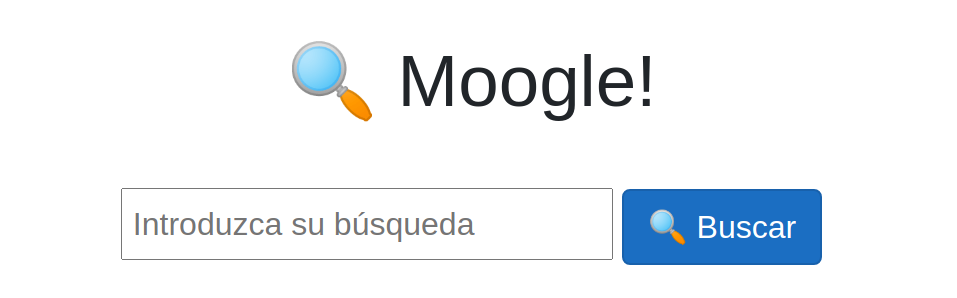
\includegraphics[width = 10 cm ]{./moogle.png}
    \caption[short]{Barra de búsqueda}
    
    \end{figure}



\end{document}